\documentclass[conference]{IEEEtran}
\IEEEoverridecommandlockouts

\usepackage{cite}
\usepackage{amsmath,amssymb,amsfonts}
\usepackage{algorithmic}
\usepackage{graphicx}
\usepackage{textcomp}
\usepackage{xcolor}
\usepackage{booktabs}
\usepackage{url}
\usepackage{hyperref}

\graphicspath{{../figures/}}

\def\BibTeX{{\rm B\kern-.05em{\sc i\kern-.025em b}\kern-.08em
    T\kern-.1667em\lower.7ex\hbox{E}\kern-.125emX}}

\begin{document}

\title{Mapping the Competitiveness Divide:\\
Unsupervised Clustering and Sparse Classification\\
of Philippine Local Government Units}

\author{
\IEEEauthorblockN{Tricci Angeles}
\IEEEauthorblockA{\textit{Department of Computer and Information Science} \\
\textit{Fordham University}\\
New York, NY, USA \\
tricciangeles13@gmail.com}
}

\maketitle

% ─────────────────────────────────────────────
\begin{abstract}
The Philippine government's Cities and Municipalities Competitiveness Index (CMCI) annually benchmarks all 1,634 local government units (LGUs) across five pillars: Economic Dynamism, Government Efficiency, Infrastructure, Resiliency, and Innovation. Despite its wide coverage, policymakers lack a data-driven framework for grouping these units into actionable tiers and for identifying the specific sub-indicators that drive or impede competitiveness. This paper addresses both problems. We apply K-Means clustering to the 2024 CMCI pillar scores and find three well-separated competitiveness tiers: \textit{Competitive Leaders} (530 LGUs, 32.4\%), \textit{Developing Mainstream} (1,059 LGUs, 64.8\%), and \textit{Critically Underserved} (45 LGUs, 2.8\%). The choice of $k{=}3$ is supported by both the elbow criterion and the peak silhouette score (0.3043). We then train an L1-penalized multinomial logistic regression on the 50 raw CMCI sub-indicators to predict cluster membership, reaching 97.9\% test accuracy and 99.3\% full-dataset accuracy. The sparse L1 solution shows that Innovation and Government Efficiency are the main differentiators of top performers, while Resiliency deficits most severely characterize the underserved tier. A model-derived watchlist flags 15 municipalities in Sulu, Lanao del Sur, and Basilan as highest-risk for underdevelopment, giving policymakers a concrete starting point for resource allocation.
\end{abstract}

\begin{IEEEkeywords}
competitiveness index, K-Means clustering, L1 logistic regression, principal component analysis, local government units, Philippines, policy analytics
\end{IEEEkeywords}

% ─────────────────────────────────────────────
\section{Introduction}

Local economic competitiveness is a multidimensional construct that determines whether a community can attract investment, deliver services, and sustain livelihoods. In the Philippine context, this is captured annually by the CMCI, published by the Department of Trade and Industry (DTI), which scores every city and municipality on five broad pillars comprising 50 granular sub-indicators. The 2024 edition covers 1,634 LGUs spanning five administrative classes, ranging from highly urbanized cities (HUCs) to sixth-class municipalities, and reveals a 60.4-point spread between the best performer (Quezon City, 60.69) and the worst (Patikul, Sulu, 0.26).

Fig.~\ref{fig:top10_lgu} illustrates this inequality. Four of the top 10 LGUs come from Metro Manila, with Quezon City leading at 60.69, but the remaining six are spread across five other provinces, showing that performance gaps exist not just between regions but within them as well. This motivates a systematic, data-driven segmentation of all 1,634 LGUs to surface structural patterns that a simple ranking cannot reveal.

\begin{figure}[htbp]
    \centering
    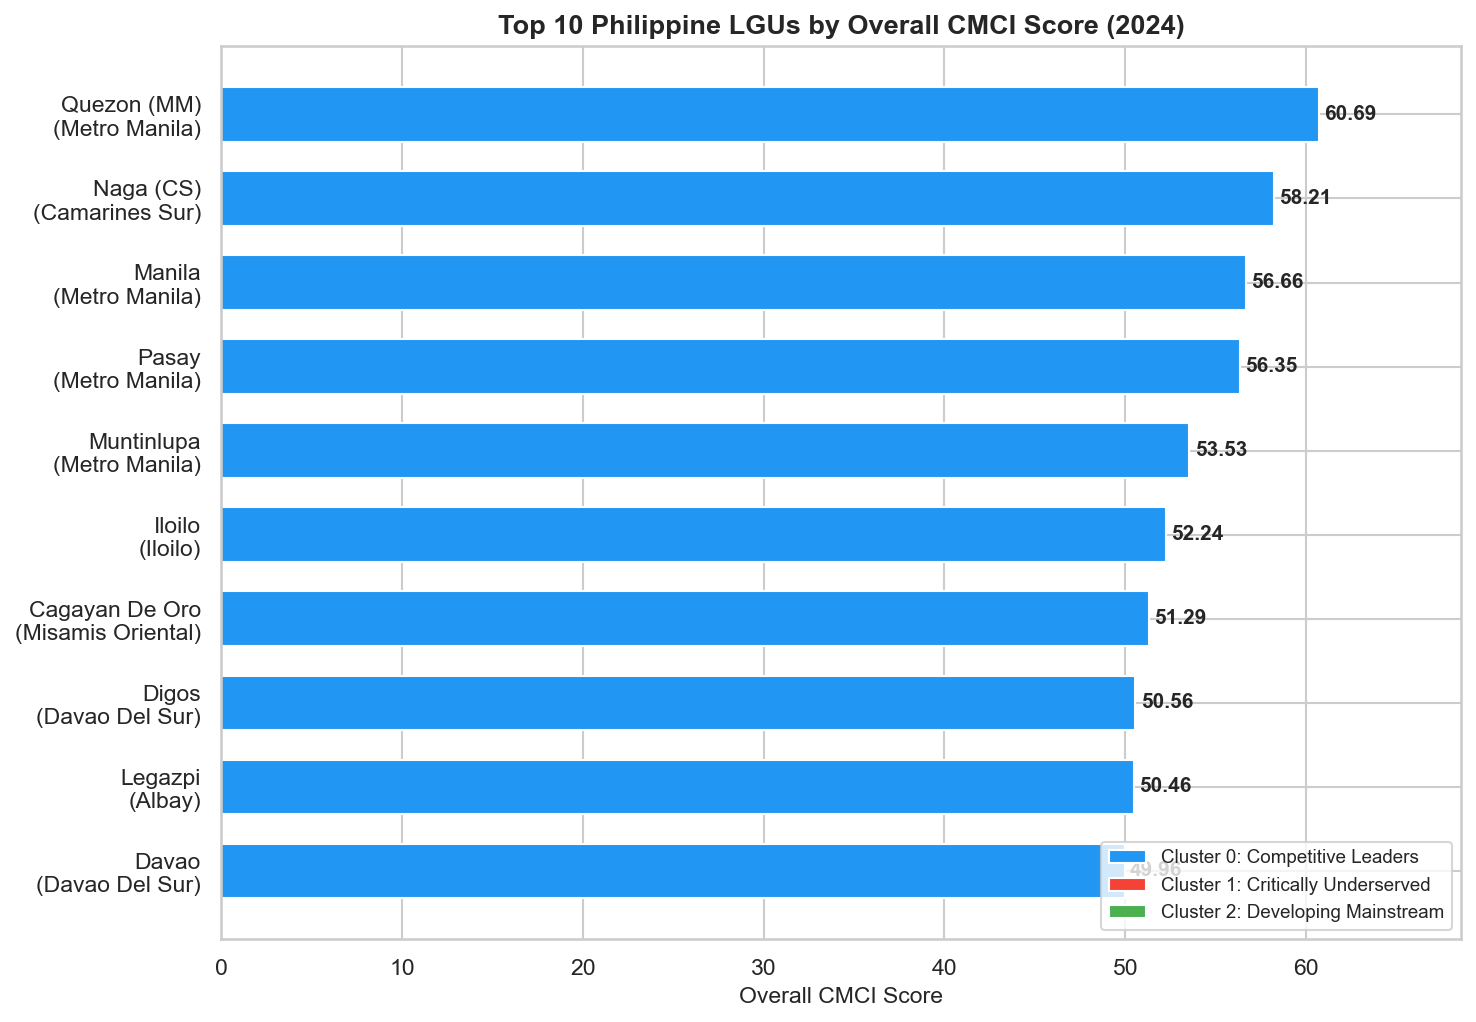
\includegraphics[width=\columnwidth]{chart_01.png}
    \caption{Top 10 Philippine LGUs by 2024 CMCI overall score. Four of the ten highest-ranked LGUs are in Metro Manila (NCR), with the remaining six spread across Camarines Sur, Iloilo, Misamis Oriental, Davao Del Sur, and Albay, showing that top performance is not confined to the capital region.}
    \label{fig:top10_lgu}
\end{figure}

Despite the richness of this dataset, CMCI rankings are typically used as a raw leaderboard rather than as inputs to a systematic segmentation. This leaves policymakers with two gaps:

\begin{enumerate}
    \item \textit{Tier identification:} How many meaningful competitiveness groups exist, and which LGUs belong to each?
    \item \textit{Driver diagnosis:} Out of 50 sub-indicators, which specific metrics most reliably separate tiers, and which interventions are therefore most likely to be effective?
\end{enumerate}

We address both questions using a two-stage machine learning pipeline. Stage 1 applies K-Means clustering to the five pillar scores to partition the 1,634 LGUs into interpretable groups. Stage 2 trains a sparse, multi-class L1 logistic regression on the 50 raw sub-indicators to (a) confirm that the cluster structure is encoded in the raw data and not just in the aggregated pillars, (b) measure the predictive importance of each sub-indicator, and (c) generate probabilities that can flag at-risk municipalities before conditions worsen.

The rest of the paper is organized as follows. Section~\ref{sec:data} describes the dataset and preprocessing. Section~\ref{sec:methods} covers the algorithms and hyperparameters. Section~\ref{sec:results} presents results and visualizations. Section~\ref{sec:discussion} interprets the findings and draws policy implications. Section~\ref{sec:conclusion} concludes.

% ─────────────────────────────────────────────
\section{Dataset and Preprocessing}
\label{sec:data}

\subsection{Data Source}

The CMCI 2024 dataset was collected from the DTI public rankings portal (\url{https://cmci.dti.gov.ph/rankings-data.php}) using \texttt{pandas.read\_html()} across five separate administrative-class pages, yielding 1,634 rows and 56 raw columns after combining them. Each row is one LGU; columns include one overall composite score, five pillar scores, and 50 sub-indicator scores.

\subsection{Administrative Classification}

Philippine LGUs are grouped into five income classes based on annual revenue and population:

\begin{itemize}
    \item \textbf{Highly Urbanized Cities (HUCs):} 33 units
    \item \textbf{Component Cities:} 116 units
    \item \textbf{1st--2nd Class Municipalities:} 509 units
    \item \textbf{3rd--4th Class Municipalities:} 660 units
    \item \textbf{5th--6th Class Municipalities:} 316 units
\end{itemize}

\subsection{Feature Structure}

The five CMCI pillars and their sub-indicators are:

\begin{itemize}
    \item \textbf{Economic Dynamism (ED):} 10 sub-indicators covering employment, business activity, local economic growth, financial deepening, and cost of living.
    \item \textbf{Government Efficiency (GE):} 11 sub-indicators covering compliance with national directives, business permitting speed, recognition of performance, and ICT adoption in governance.
    \item \textbf{Infrastructure (IF):} 10 sub-indicators covering road networks, utilities, transportation access, port proximity, and internet capability.
    \item \textbf{Resiliency (RE):} 9 sub-indicators covering disaster risk plans, early warning systems, emergency infrastructure, health capacity, and sanitation.
    \item \textbf{Innovation (IN):} 10 sub-indicators covering STEM graduates, ICT plans, new technology adoption, R\&D expenditure, and start-up facilities.
\end{itemize}

Fig.~\ref{fig:pillar_dist} shows the score distribution for each pillar across all 1,634 LGUs. All five are right-skewed, meaning most municipalities score low and a small number score high. This skew is part of what makes a data-driven grouping more useful than a simple ranking.

\begin{figure*}[t]
    \centering
    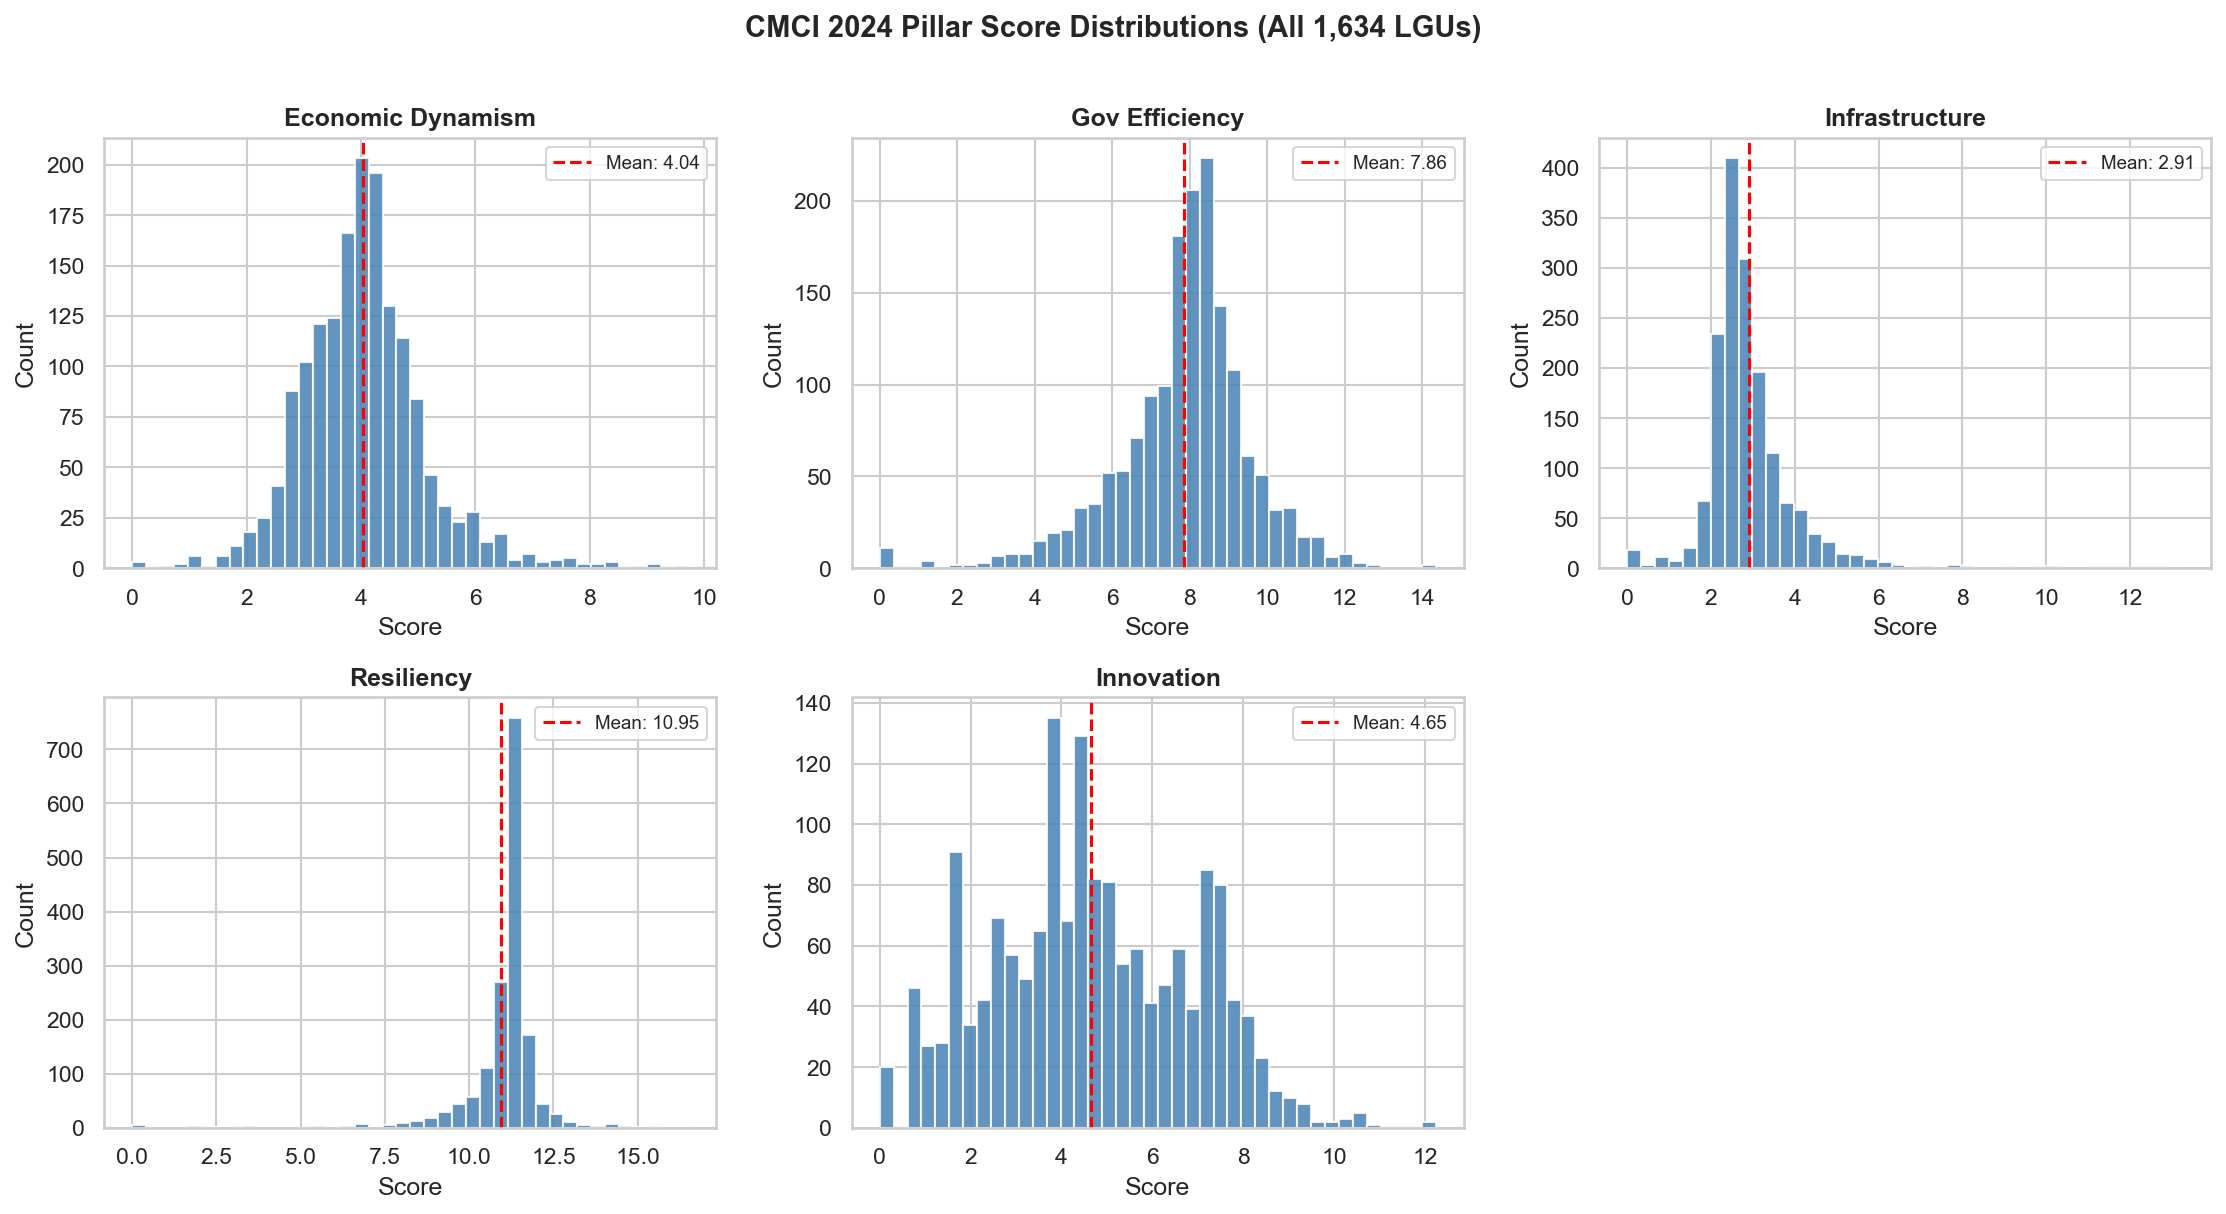
\includegraphics[width=\textwidth]{chart_03.png}
    \caption{Distribution of 2024 CMCI pillar scores across all 1,634 LGUs (40 bins each). All five pillars are right-skewed, with most municipalities bunched at the lower end and a thin tail of high performers, reflecting the well-known development inequality across Philippine regions.}
    \label{fig:pillar_dist}
\end{figure*}

\subsection{Preprocessing Pipeline}

\textbf{Cleaning and type conversion.} Column names were standardized to snake\_case. All score columns were cast to \texttt{float64}. A categorical \texttt{lgu\_type} field and a \texttt{Region} field covering 17 Philippine administrative regions were added from structural metadata.

\textbf{Standardization for clustering.} The five pillar scores were standardized using \texttt{StandardScaler} (zero mean, unit variance), producing a $1634 \times 5$ matrix $\mathbf{X}_{\text{scaled}}$ used for K-Means and PCA.

\textbf{Standardization for classification.} The 50 raw sub-indicator scores were standardized separately using \texttt{StandardScaler} into a $1634 \times 50$ matrix $\mathbf{X}_{50}$ for logistic regression, which the SAGA solver requires with L1 penalty.

\textbf{Train/test split.} A stratified 80/20 split was applied using cluster labels as the stratification variable, giving 1,307 training samples and 327 test samples. Stratification was necessary because the smallest cluster has only 45 LGUs (2.8\%), and a random split could easily leave it underrepresented in either set.

% ─────────────────────────────────────────────
\section{Methodology}
\label{sec:methods}

\subsection{Stage 1: K-Means Clustering}

K-Means partitions $n$ observations into $k$ clusters by minimizing the within-cluster sum of squared Euclidean distances (inertia):

\begin{equation}
    J = \sum_{j=1}^{k} \sum_{\mathbf{x}_i \in C_j} \|\mathbf{x}_i - \boldsymbol{\mu}_j\|^2
\end{equation}

where $\boldsymbol{\mu}_j$ is the centroid of cluster $C_j$. We used scikit-learn's \texttt{KMeans} with Lloyd's algorithm, \texttt{n\_init=10} random restarts, and \texttt{random\_state=42}.

\textbf{Choosing $k$.} We tested values from 2 to 10 using two criteria:

\begin{itemize}
    \item \textit{Elbow criterion:} Inertia drops sharply from $k{=}2$ to $k{=}3$ and levels off after that, placing the elbow at $k{=}3$.
    \item \textit{Silhouette score:} The mean silhouette coefficient $s = \frac{b - a}{\max(a, b)}$, where $a$ is intra-cluster distance and $b$ is the nearest inter-cluster distance, peaks at $k{=}3$ with $s{=}0.3043$ and falls for every larger value.
\end{itemize}

Both criteria pointed to $k{=}3$, as shown in Fig.~\ref{fig:elbow}, confirming that three tiers are the natural grouping for this data.

\begin{figure}[htbp]
    \centering
    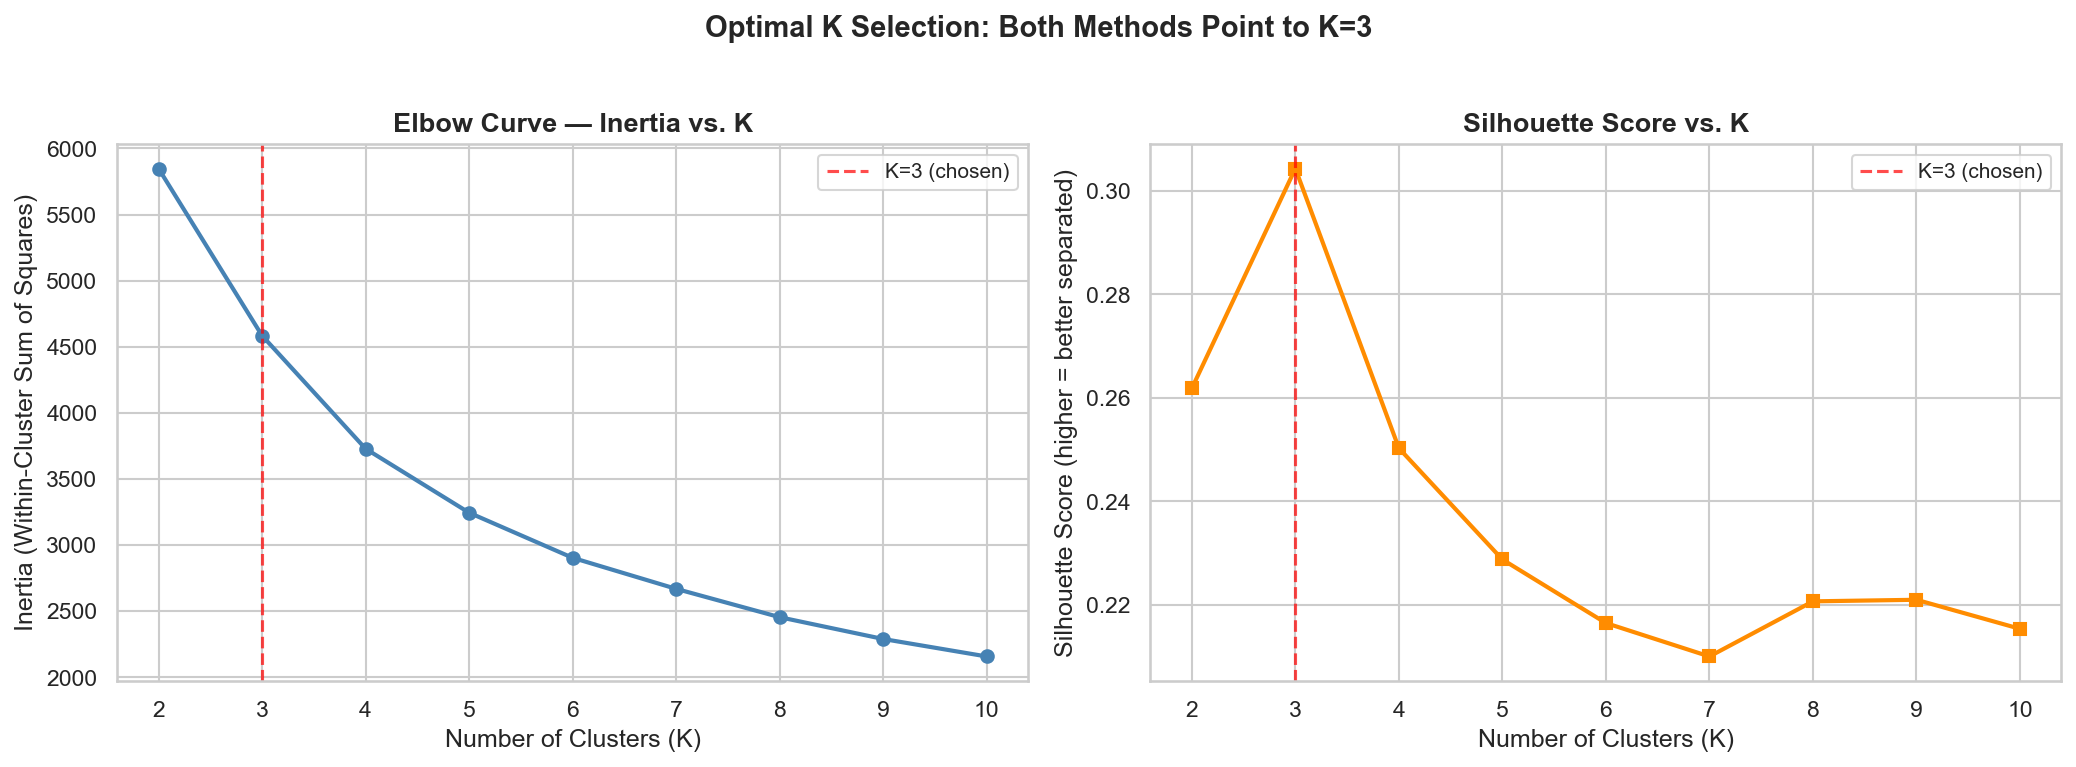
\includegraphics[width=\columnwidth]{chart_04.png}
    \caption{K-Means model selection for $k = 2$ to $10$. Left: the elbow curve shows a sharp drop in inertia at $k{=}3$ that flattens for larger $k$. Right: the silhouette score peaks at $k{=}3$ (0.3043) and declines for every value above it, confirming three clusters as the best partition.}
    \label{fig:elbow}
\end{figure}

\subsection{Stage 2: PCA Visualization}

To visually check how well the clusters separate, we applied Principal Component Analysis (\texttt{PCA}, $d{=}2$) to $\mathbf{X}_{\text{scaled}}$. The two principal components together explained 75.9\% of total variance (PC1: 58.8\%, PC2: 17.1\%), giving a reasonable 2D view of the original five-dimensional pillar space.

\subsection{Stage 3: L1 Logistic Regression}

After assigning cluster labels, we trained a multi-class L1-penalized logistic regression using \texttt{LogisticRegressionCV} with the SAGA solver on the $\mathbf{X}_{50}$ sub-indicator matrix to predict cluster membership. The objective is:

\begin{equation}
    \min_{\mathbf{W}} \; -\frac{1}{n}\sum_{i=1}^{n} \log p(y_i \mid \mathbf{x}_i; \mathbf{W}) + \frac{1}{C} \|\mathbf{W}\|_1
\end{equation}

Key hyperparameters:

\begin{itemize}
    \item \texttt{Cs=20}: 20 regularization strength values tested during cross-validation.
    \item \texttt{cv=5}: 5-fold cross-validation to pick the best $C$.
    \item \texttt{penalty='l1'}: Produces a sparse solution by zeroing out weak features.
    \item \texttt{solver='saga'}: The only scikit-learn solver that supports L1 with multi-class problems.
    \item \texttt{class\_weight='balanced'}: Adjusts for class imbalance since Cluster 1 is only 2.8\% of the data.
    \item \texttt{max\_iter=5000}: Enough iterations for SAGA to converge at this dimensionality.
\end{itemize}

L1 was chosen over L2 because it drives many coefficient weights to exactly zero, making it easy to read off which sub-indicators actually matter for each tier.

% ─────────────────────────────────────────────
\section{Results}
\label{sec:results}

\subsection{Cluster Identification and Profiles}

Table~\ref{tab:cluster_summary} shows the three clusters' sizes and average pillar scores. The names (\textit{Competitive Leaders}, \textit{Developing Mainstream}, and \textit{Critically Underserved}) were assigned after the fact based on overall score.

\begin{table}[htbp]
\caption{K-Means Cluster Profiles (2024 CMCI, $k=3$)}
\label{tab:cluster_summary}
\centering
\begin{tabular}{lccc}
\toprule
\textbf{Metric} & \textbf{Cluster 0} & \textbf{Cluster 1} & \textbf{Cluster 2} \\
 & \textit{Leaders} & \textit{Underserved} & \textit{Mainstream} \\
\midrule
\textbf{Count} & 530 (32.4\%) & 45 (2.8\%) & 1,059 (64.8\%) \\
\midrule
Economic Dynamism & 4.78 & 2.62 & 3.74 \\
Gov. Efficiency & 9.25 & 2.86 & 7.38 \\
Infrastructure & 3.77 & 1.45 & 2.54 \\
Resiliency & 11.65 & 4.13 & 10.89 \\
Innovation & 6.81 & 1.30 & 3.72 \\
\midrule
\textbf{Overall Score} & \textbf{36.26} & \textbf{12.36} & \textbf{28.26} \\
\bottomrule
\end{tabular}
\end{table}

The Critically Underserved cluster (Cluster 1) does not just underperform on one pillar; it scores near the bottom across all five. The heatmap in Fig.~\ref{fig:cluster_heatmap} and the radar chart in Fig.~\ref{fig:radar} make this visually clear, and Fig.~\ref{fig:boxplot} shows that the three clusters' overall score distributions barely overlap.

\begin{figure}[htbp]
    \centering
    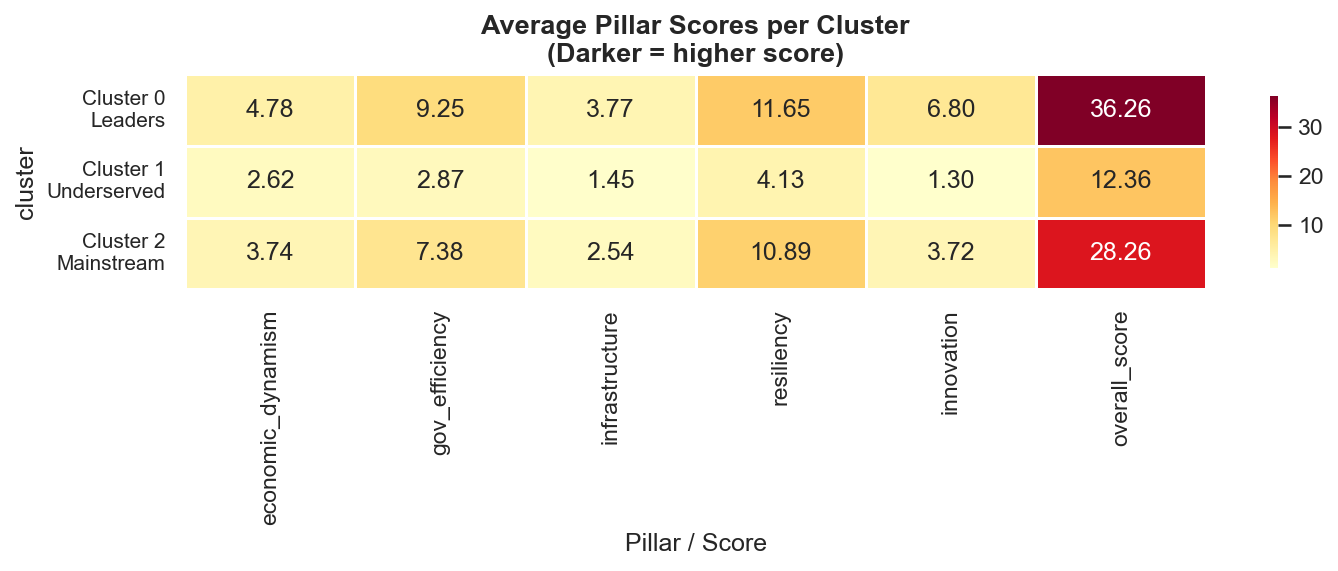
\includegraphics[width=\columnwidth]{chart_06.png}
    \caption{Cluster profiles heatmap showing average pillar and overall scores for each of the three K-Means clusters. Cluster 1 (Critically Underserved) registers low values across every pillar, not just one, pointing to compound deprivation. Cluster 0 (Leaders) scores highest on Innovation and Government Efficiency.}
    \label{fig:cluster_heatmap}
\end{figure}

\begin{figure}[htbp]
    \centering
    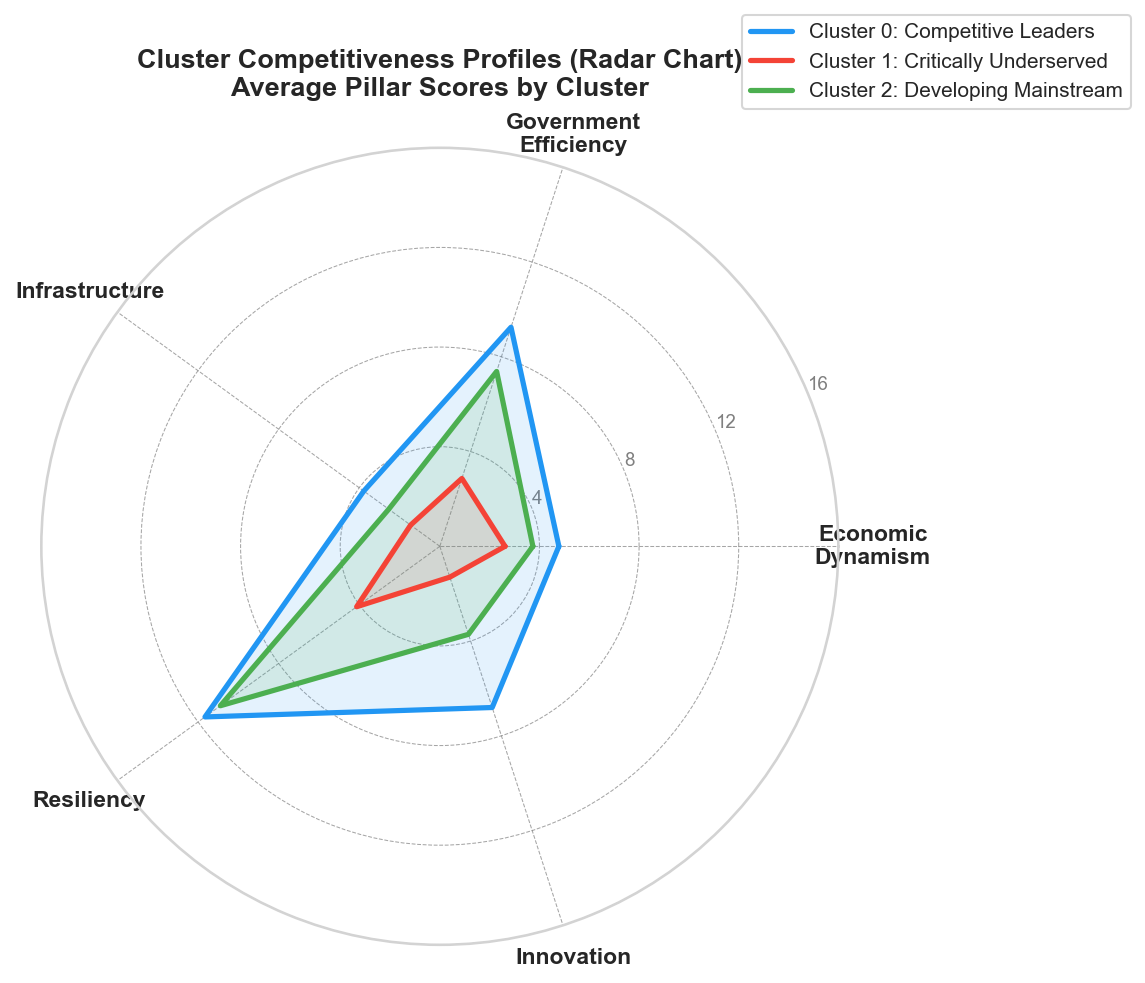
\includegraphics[width=\columnwidth]{chart_08.png}
    \caption{Radar chart comparing the five-pillar profiles of the three competitiveness clusters. The area enclosed by each polygon reflects overall competitiveness. Cluster 0 (Leaders) dominates all axes, while Cluster 1 (Underserved) collapses nearly to the center, showing that this group is weak across every dimension at once.}
    \label{fig:radar}
\end{figure}

\begin{figure}[htbp]
    \centering
    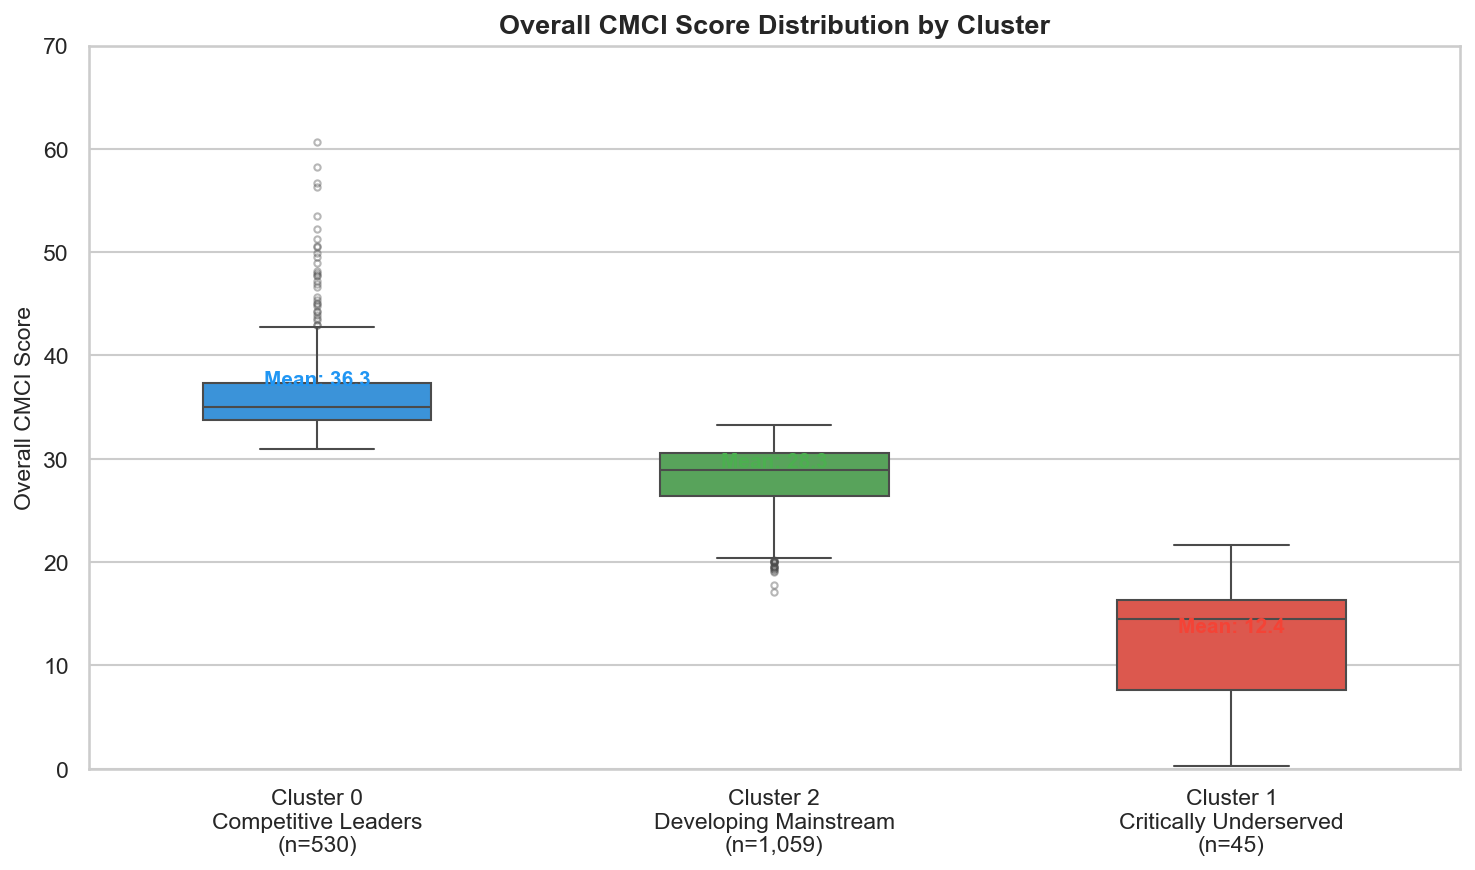
\includegraphics[width=\columnwidth]{chart_09.png}
    \caption{Box plot of overall CMCI scores by cluster. Cluster 0 (Leaders) spans roughly 33 to 61, Cluster 2 (Mainstream) spans 22 to 35, and Cluster 1 (Underserved) is capped near 22. The limited overlap confirms that K-Means found three genuinely distinct performance groups.}
    \label{fig:boxplot}
\end{figure}

\subsection{K Selection Validation}

Table~\ref{tab:kmeans_selection} reports inertia and silhouette scores for $k{=}2$ through $k{=}10$. The silhouette score peaks at $k{=}3$ and falls for every larger value, while the sharpest drop in inertia also occurs at the $k{=}2$ to $k{=}3$ step (Fig.~\ref{fig:elbow}).

\begin{table}[htbp]
\caption{K-Means Model Selection ($k = 2$ to $10$)}
\label{tab:kmeans_selection}
\centering
\begin{tabular}{ccc}
\toprule
\textbf{$k$} & \textbf{Inertia} & \textbf{Silhouette Score} \\
\midrule
2  & 5,847.87 & 0.2618 \\
\textbf{3}  & \textbf{4,583.89} & \textbf{0.3043} \\
4  & 3,728.23 & 0.2503 \\
5  & 3,244.27 & 0.2288 \\
6  & 2,903.01 & 0.2165 \\
7  & 2,668.13 & 0.2100 \\
8  & 2,453.84 & 0.2207 \\
9  & 2,288.85 & 0.2210 \\
10 & 2,156.56 & 0.2153 \\
\bottomrule
\end{tabular}
\end{table}

\subsection{PCA Cluster Visualization}

Fig.~\ref{fig:pca} plots all 1,634 LGUs in the 2D PCA space. The three clusters occupy clearly separate regions with little overlap. Cluster 1 (Critically Underserved) sits as a compact, isolated group at the far negative end of PC1, which is consistent with its low scores across all pillars. PC1 (58.8\% of variance) mainly captures overall competitiveness level; PC2 (17.1\%) separates the Innovation and Governance profile of Cluster 0 from the Resiliency-leaning profile of Cluster 2.

\begin{figure}[htbp]
    \centering
    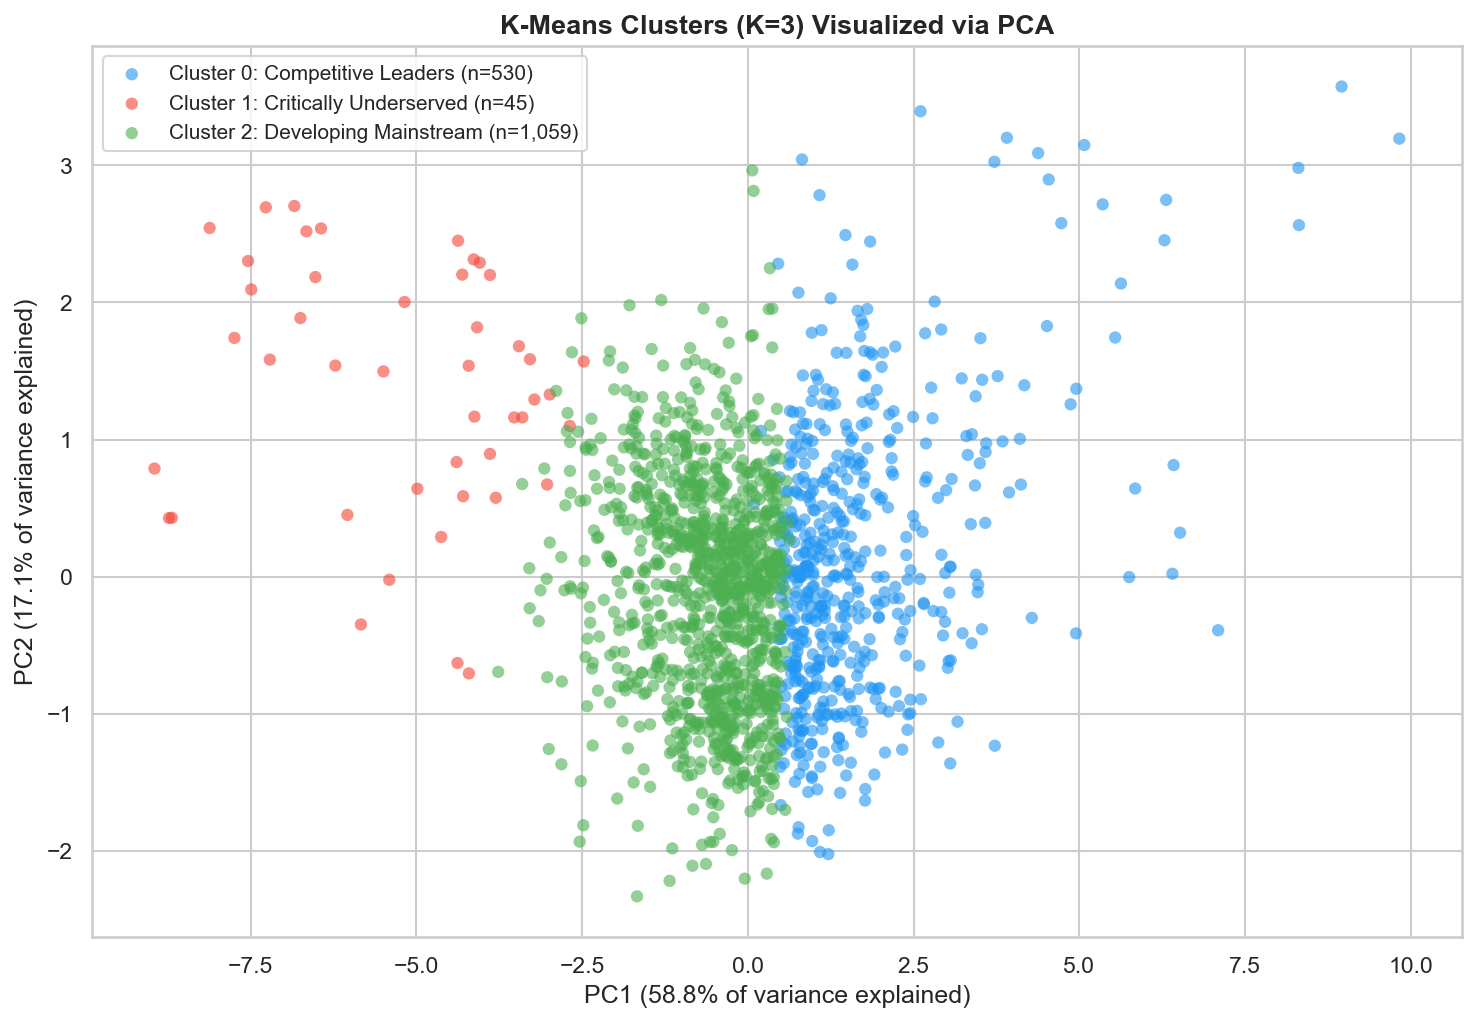
\includegraphics[width=\columnwidth]{chart_05.png}
    \caption{PCA scatter plot of all 1,634 LGUs colored by cluster. PC1 and PC2 together capture 75.9\% of variance in the five-pillar space. The three clusters sit in well-separated regions, with Cluster 1 (Critically Underserved, red) forming a tight isolated group at the lower left and Cluster 0 (Leaders, blue) in the upper right.}
    \label{fig:pca}
\end{figure}

\subsection{Classification Performance}

Table~\ref{tab:classification} reports precision, recall, and F1-score on the held-out test set ($n{=}327$). Fig.~\ref{fig:confusion} shows the confusion matrix.

\begin{table}[htbp]
\caption{L1 Logistic Regression Test Set Results ($n=327$)}
\label{tab:classification}
\centering
\begin{tabular}{lcccc}
\toprule
\textbf{Cluster} & \textbf{Precision} & \textbf{Recall} & \textbf{F1} & \textbf{Support} \\
\midrule
0 (Leaders)     & 0.97 & 0.97 & 0.97 & 106 \\
1 (Underserved) & 0.90 & 1.00 & 0.95 & 9 \\
2 (Mainstream)  & 0.99 & 0.98 & 0.98 & 212 \\
\midrule
Macro Average   & 0.95 & 0.98 & 0.97 & 327 \\
Weighted Avg.   & 0.98 & 0.98 & 0.98 & 327 \\
\midrule
\textbf{Overall Accuracy} & \multicolumn{4}{c}{\textbf{97.9\%}} \\
\bottomrule
\end{tabular}
\end{table}

\begin{figure}[htbp]
    \centering
    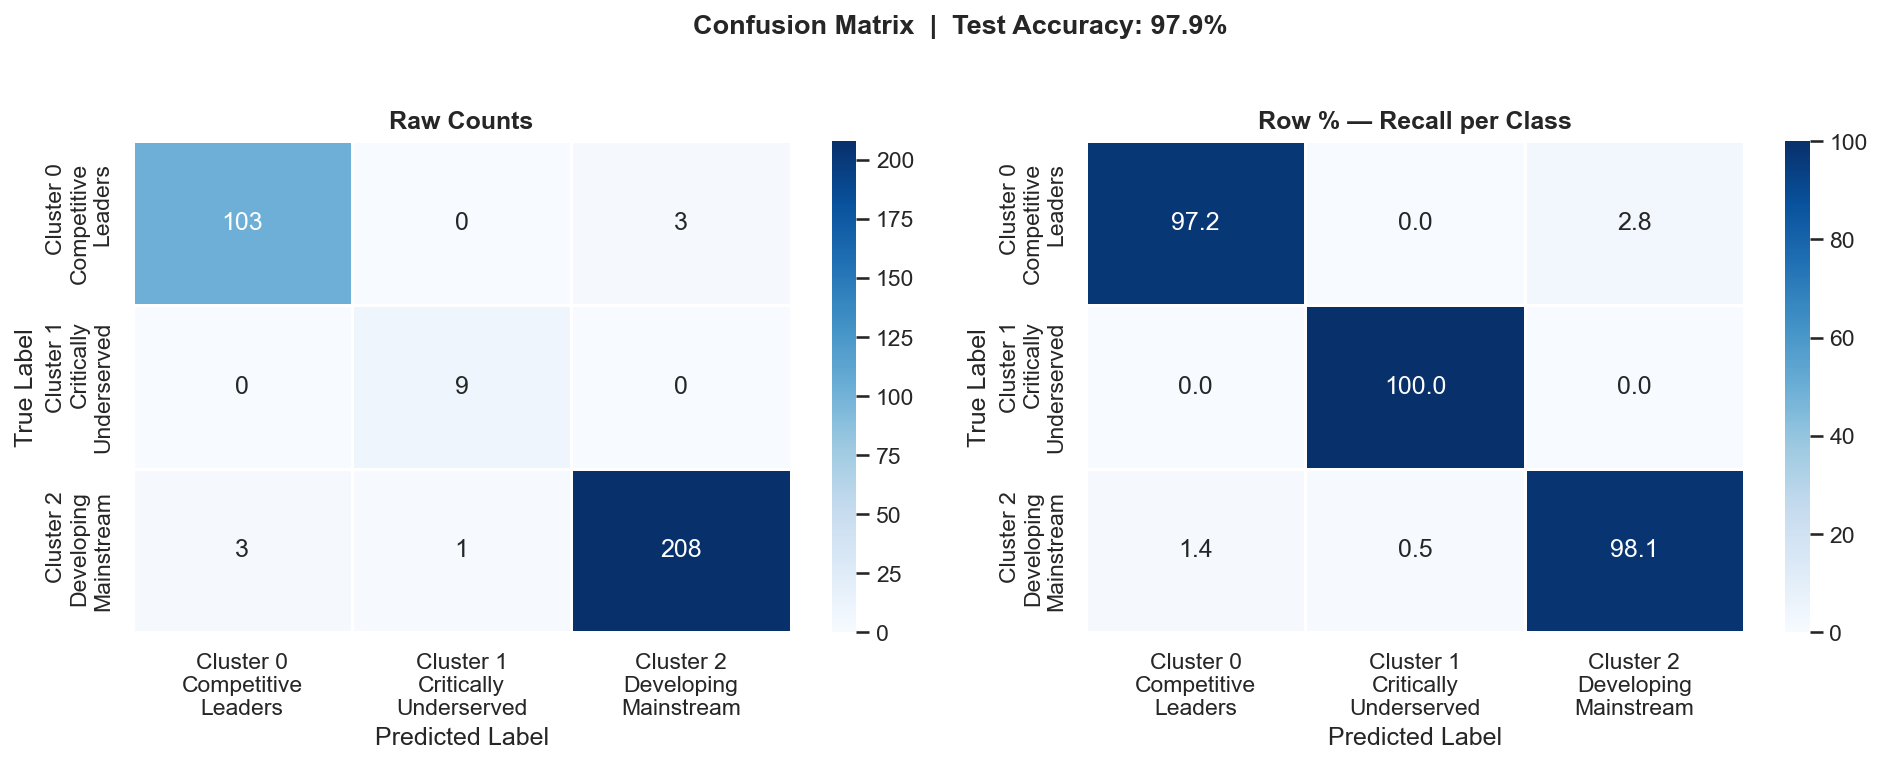
\includegraphics[width=\columnwidth]{chart_10.png}
    \caption{Confusion matrix for the L1 logistic regression on the 327-LGU test set (left: raw counts; right: row percentages). The diagonal dominates both panels. Cluster 1 (Critically Underserved) reaches 100\% recall, meaning no at-risk municipality was missed, which is the most important outcome for any policy-targeting use of this model.}
    \label{fig:confusion}
\end{figure}

The Critically Underserved cluster reaches a perfect recall of 1.00 on the test set despite making up only 2.8\% of the data. This means the model catches every at-risk municipality without false negatives, which matters greatly in a policy setting where overlooking a high-need community has real consequences. Full-dataset accuracy is 99.3\% (1,623 of 1,634 LGUs correctly classified).

\subsection{Feature Sparsity and Sub-Indicator Importance}

The L1 penalty zeroed out different numbers of the 50 sub-indicators for each class:

\begin{itemize}
    \item Cluster 0 (Leaders): 45 of 50 features active (90\%)
    \item Cluster 1 (Underserved): 19 of 50 features active (38\%)
    \item Cluster 2 (Mainstream): 16 of 50 features active (32\%)
\end{itemize}

This difference makes sense: reaching the Leaders tier requires strong performance across nearly everything, while belonging to the underserved group is driven by a narrower set of failures. Figs.~\ref{fig:top15} and~\ref{fig:pillar_importance} show which sub-indicators and pillars carry the most weight for each cluster.

\begin{figure*}[t]
    \centering
    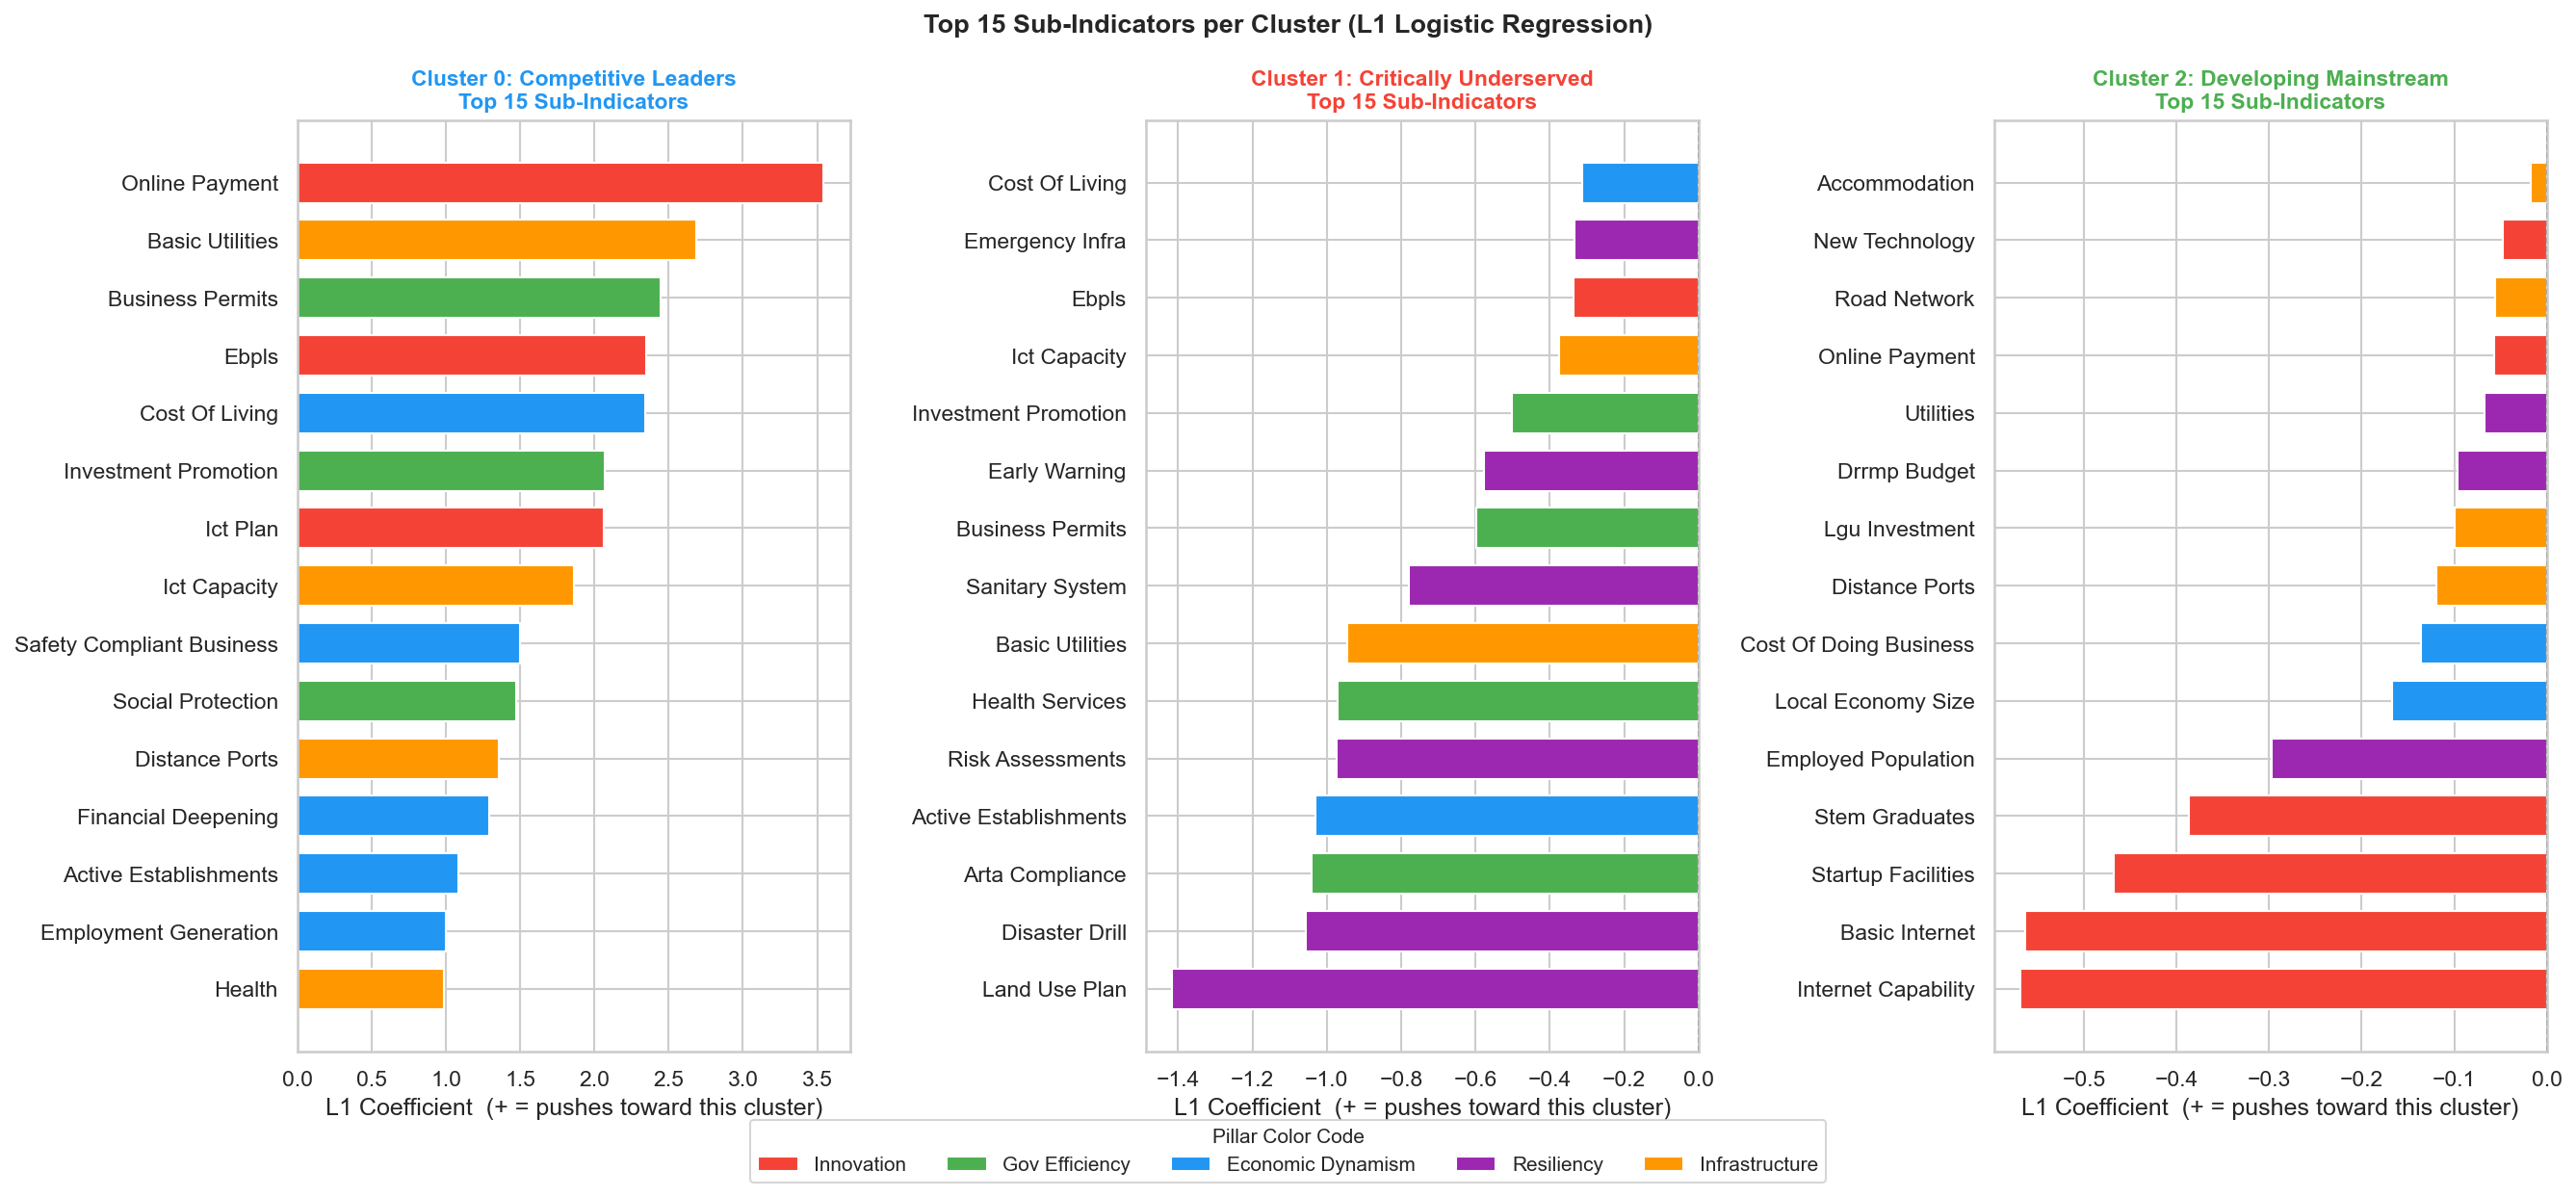
\includegraphics[width=\textwidth]{chart_11.png}
    \caption{Top 15 most predictive sub-indicators for each cluster, ranked by absolute L1 coefficient. Cluster 0 (Leaders) draws on a wide range of Innovation and Government Efficiency metrics. Cluster 1 (Underserved) is shaped mainly by deficits in health capacity, internet access, and governance. Cluster 2 (Mainstream) is most sensitive to Resiliency sub-indicators.}
    \label{fig:top15}
\end{figure*}

\begin{figure}[htbp]
    \centering
    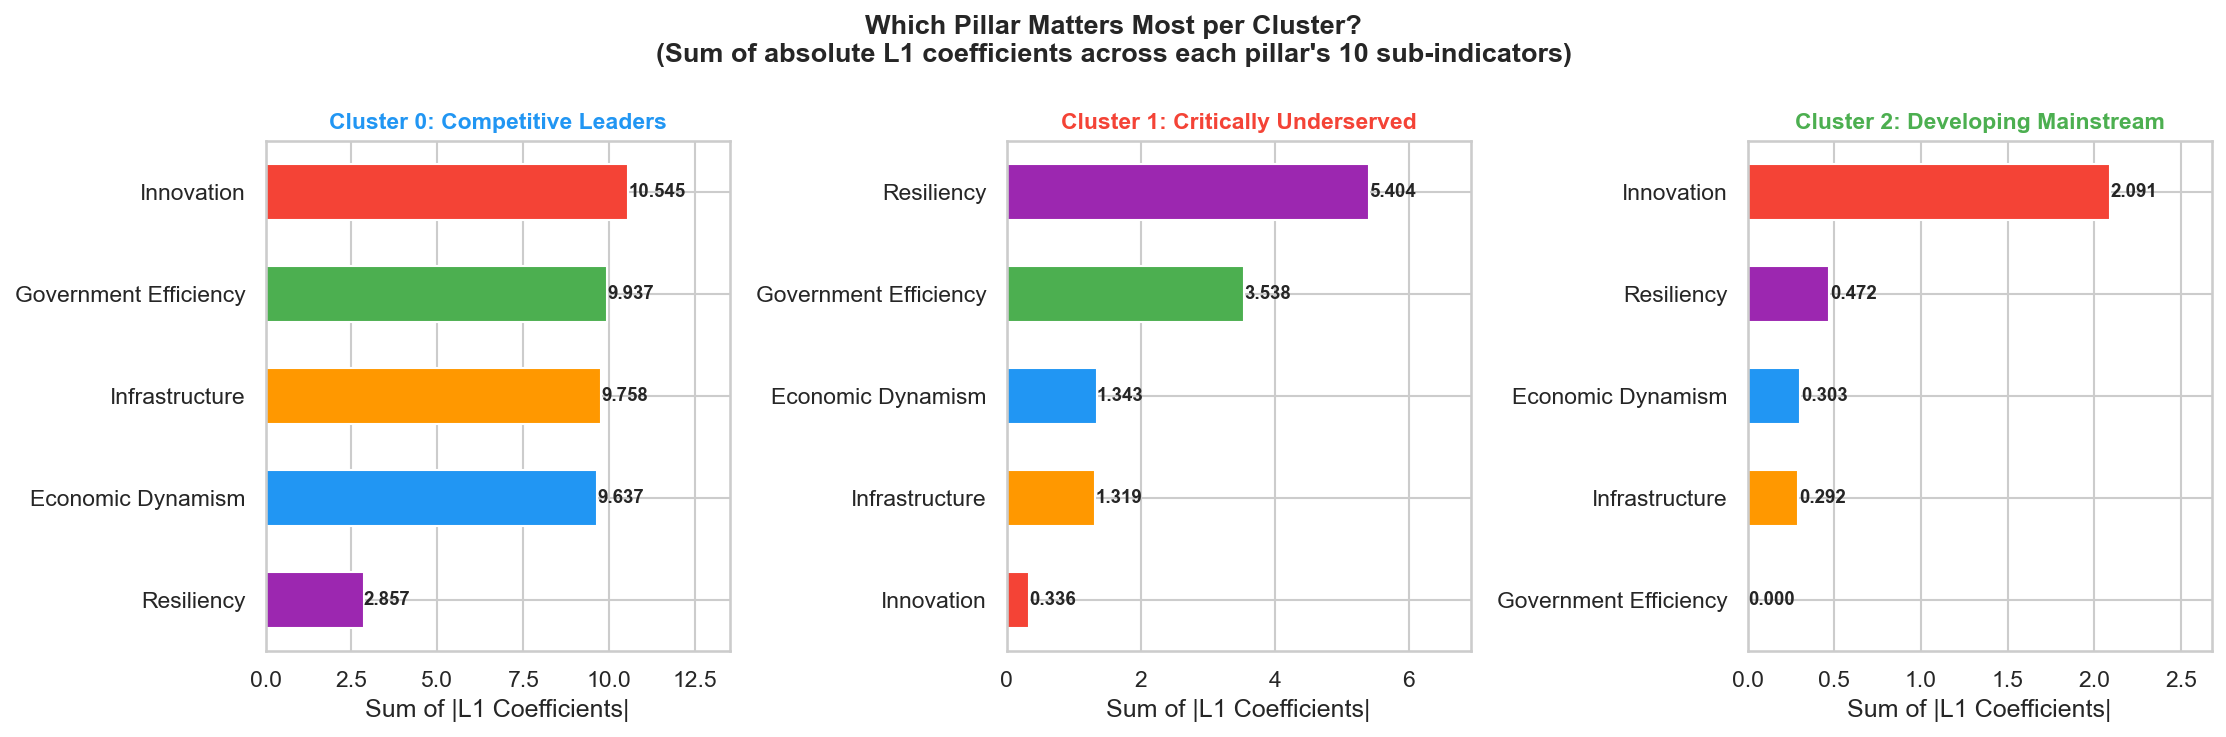
\includegraphics[width=\columnwidth]{chart_12.png}
    \caption{Pillar-level feature importance, computed as the sum of absolute L1 coefficients per pillar per cluster. Innovation (10.54) is the strongest predictor of Cluster 0 (Leaders), while Resiliency (5.40) most strongly characterizes Cluster 1 (Underserved). Infrastructure is never the leading pillar: it ranks third for Cluster 0 (9.76) and only fourth of five for Clusters 1 (1.32) and 2 (0.29).}
    \label{fig:pillar_importance}
\end{figure}

Grouping coefficient magnitudes by pillar gives the following ranking:

\begin{itemize}
    \item \textbf{Cluster 0 (Leaders):} Innovation (10.54) $>$ Government Efficiency (9.94) $>$ Infrastructure (9.76)
    \item \textbf{Cluster 1 (Underserved):} Resiliency (5.40) $>$ Government Efficiency (3.54)
    \item \textbf{Cluster 2 (Mainstream):} Innovation (2.09) is the top predictor for this tier
\end{itemize}

\subsection{At-Risk Municipality Watchlist}

Fig.~\ref{fig:flags_underserved} shows which sub-indicators most strongly signal that an LGU belongs to Cluster 1, while Fig.~\ref{fig:atrisk} ranks all LGUs by their predicted probability of being Critically Underserved.

\begin{figure}[htbp]
    \centering
    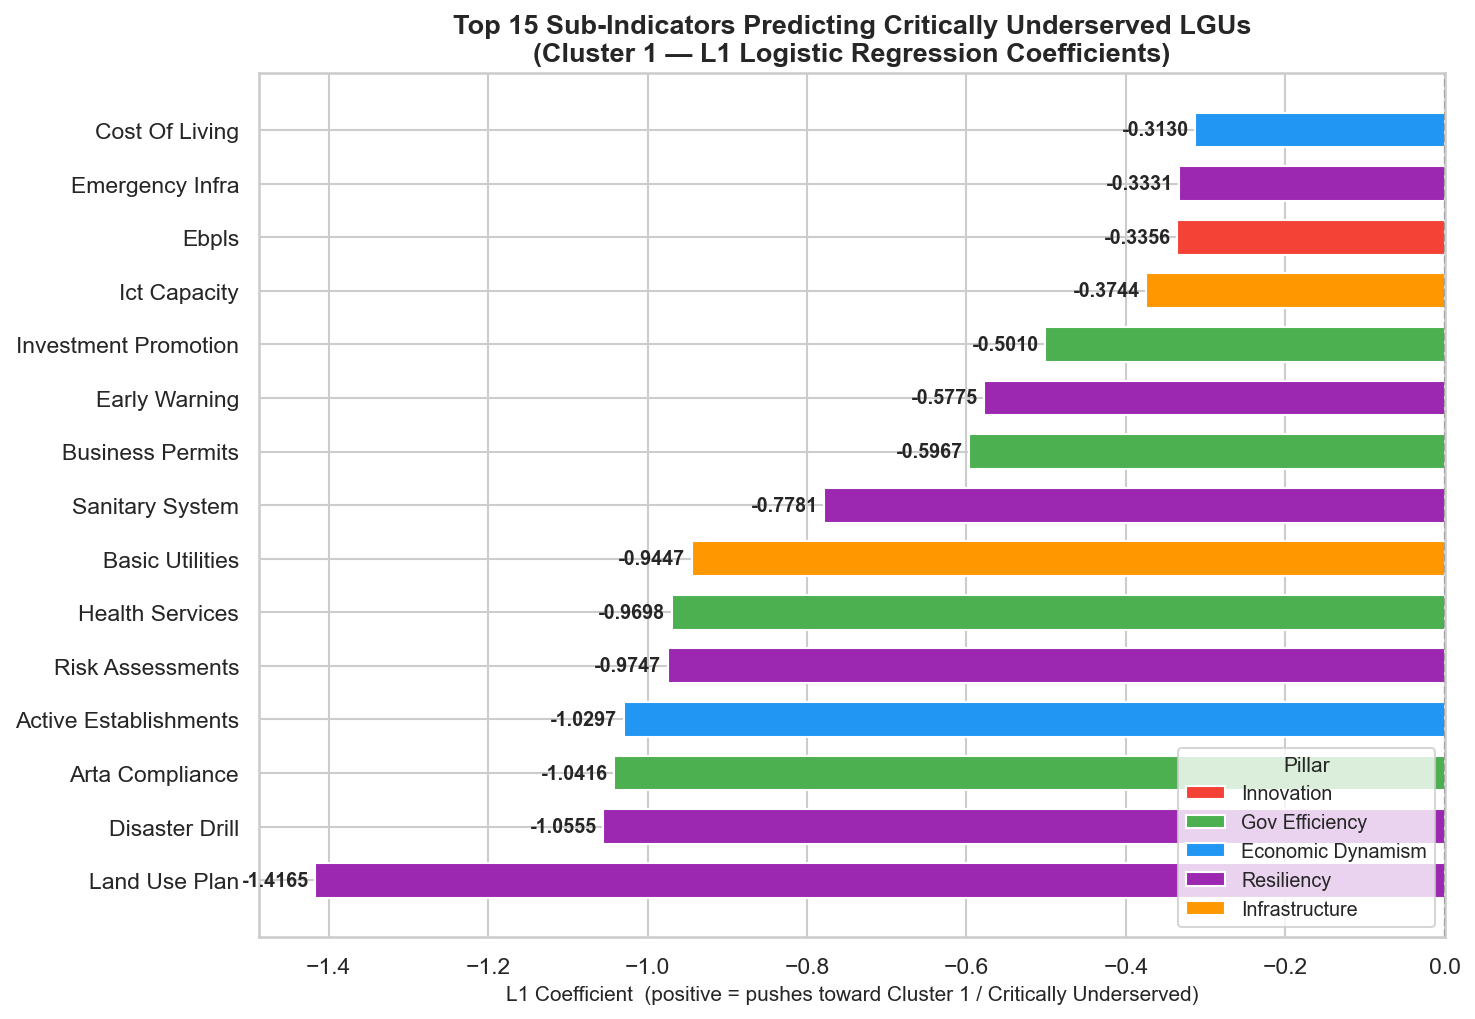
\includegraphics[width=\columnwidth]{chart_13.png}
    \caption{Sub-indicators with the strongest association with Critically Underserved (Cluster 1) membership, based on L1 regression coefficients. Deficits in health service capacity, internet availability, and STEM education are the clearest warning signals, consistent with the broad nature of deprivation in the lowest-performing municipalities.}
    \label{fig:flags_underserved}
\end{figure}

\begin{figure}[htbp]
    \centering
    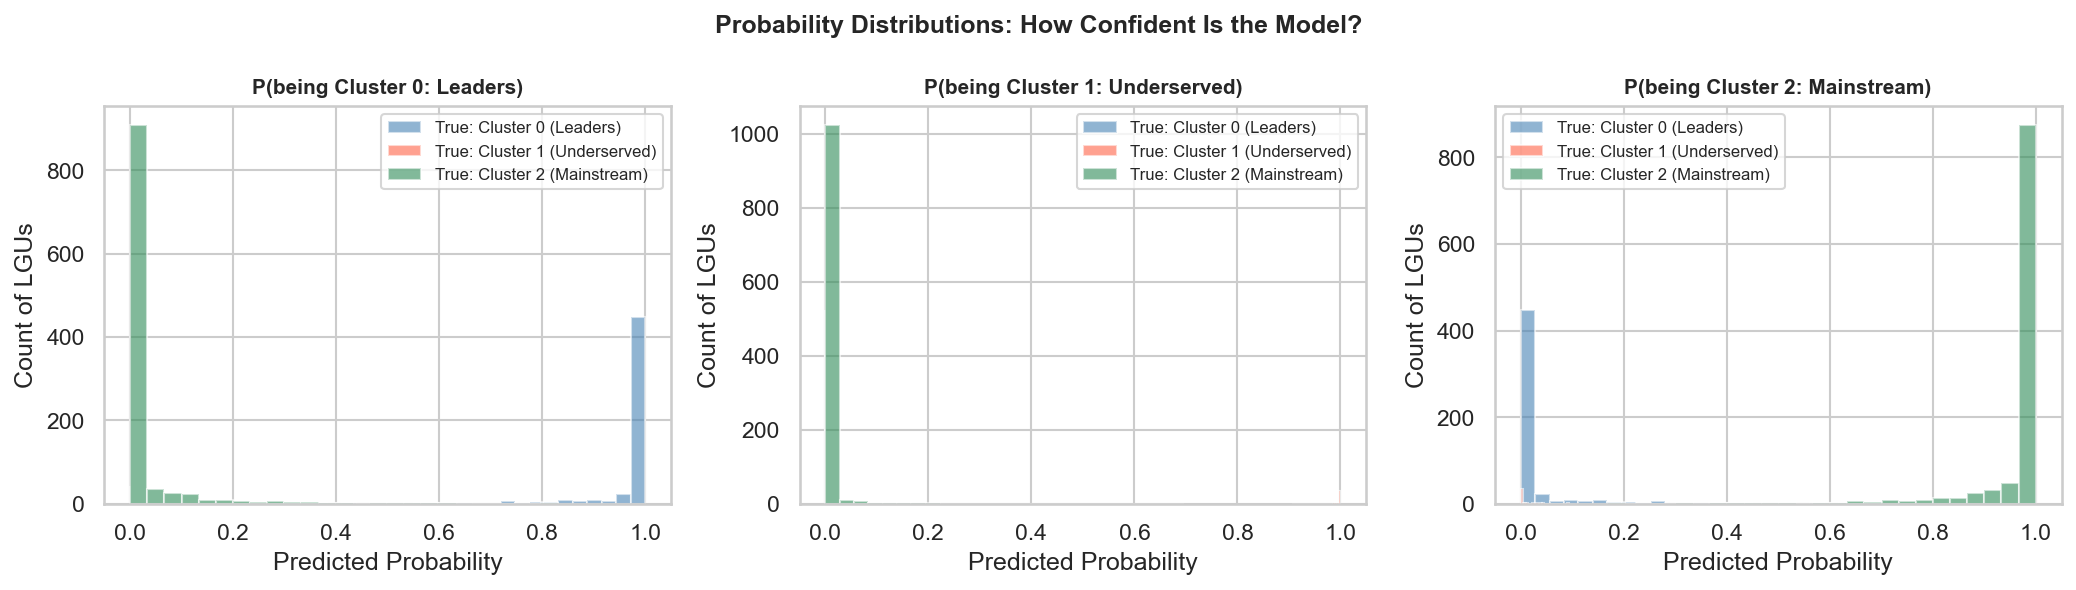
\includegraphics[width=\columnwidth]{chart_14.png}
    \caption{At-risk LGU watchlist. Top: the 15 municipalities with the highest predicted probability of Cluster 1 (Critically Underserved) membership, all located in Sulu, Lanao del Sur, and Basilan (BARMM), each with a predicted probability of exactly $P{=}1.0$. Bottom: probability histogram showing the model's confidence, with true Cluster 1 LGUs bunched sharply near 1.0 and no ambiguous predictions in the middle.}
    \label{fig:atrisk}
\end{figure}

Using predicted probabilities of Cluster 1 membership, we ranked all 1,634 LGUs to build a watchlist of the 15 most at-risk municipalities. All 15 are in Sulu, Lanao del Sur, and Basilan in the BARMM (Bangsamoro Autonomous Region in Muslim Mindanao), each with a predicted probability of exactly 1.0, meaning the model has no uncertainty about their at-risk status.

\subsection{Geographic and Administrative Patterns}

Fig.~\ref{fig:lgu_type} shows the administrative-class breakdown within each cluster. HUCs and Component Cities are concentrated in Cluster 0 (Leaders), while Cluster 1 (Underserved) is made up mostly of 3rd- and 4th-class municipalities (25 of 45 LGUs), with 5th- and 6th-class municipalities (18 of 45) also well represented. Cluster 2 (Mainstream) is the most mixed, with municipalities from all income classes.

\begin{figure}[htbp]
    \centering
    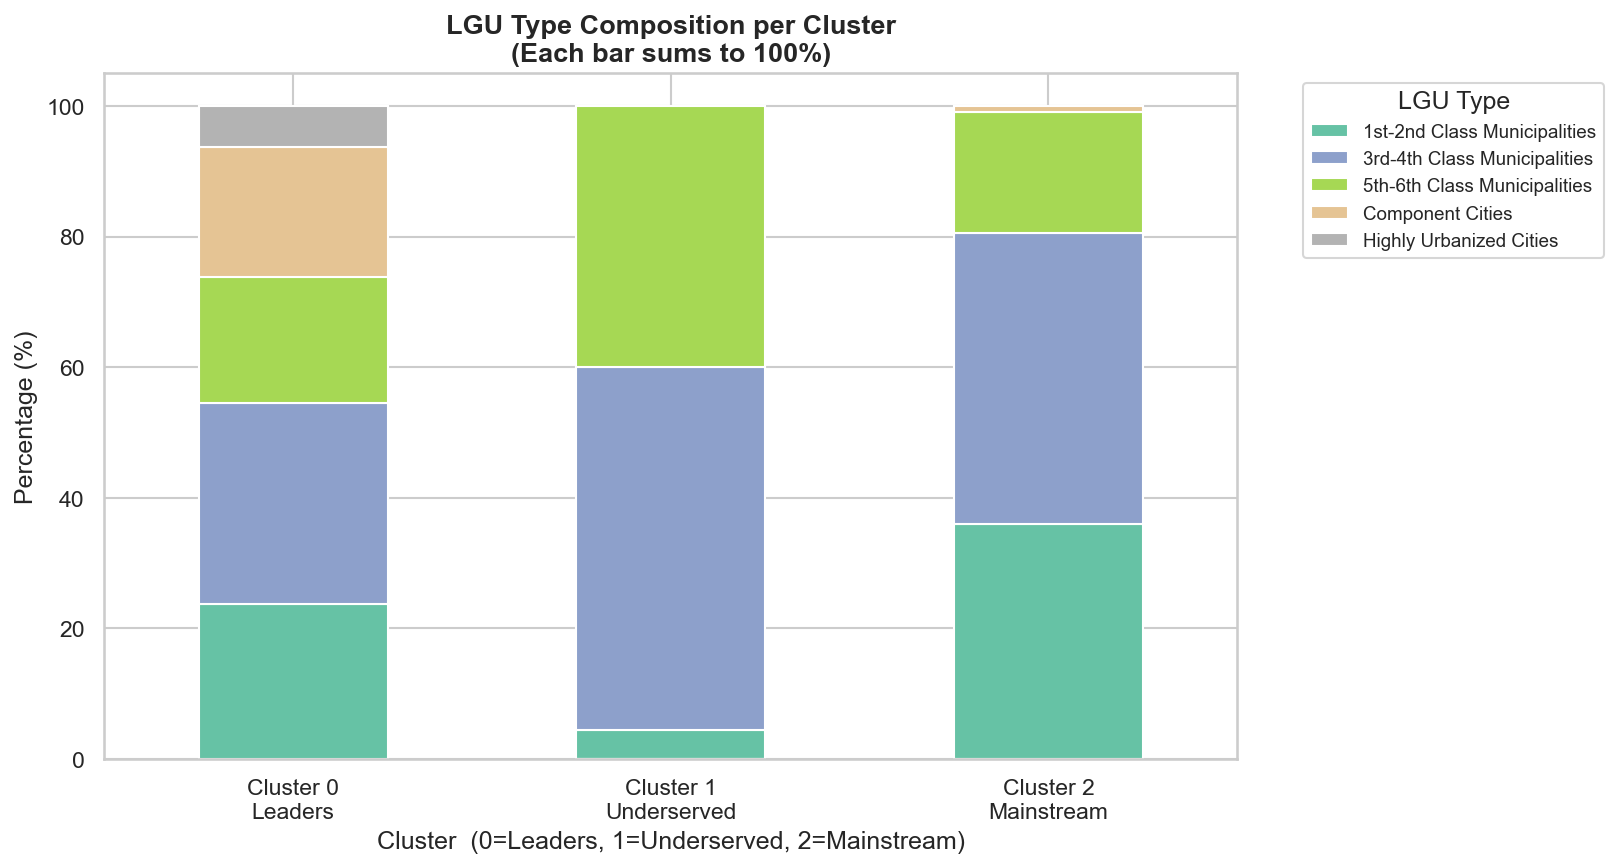
\includegraphics[width=\columnwidth]{chart_07.png}
    \caption{Administrative-class composition within each K-Means cluster. Cluster 0 (Competitive Leaders) is dominated by Highly Urbanized Cities and Component Cities. Cluster 1 (Critically Underserved) is made up primarily of 3rd- and 4th-class municipalities (25 of 45), followed by 5th- and 6th-class municipalities (18 of 45). Administrative income class turns out to be a reliable proxy for competitiveness tier.}
    \label{fig:lgu_type}
\end{figure}

Fig.~\ref{fig:top10_subind} offers a look at the other end of the spectrum. The heatmap of top sub-indicators for the 10 best-scoring LGUs shows uniformly high values across the board, confirming that top performance in this index is broad-based and not driven by strength in just one area.

\begin{figure*}[t]
    \centering
    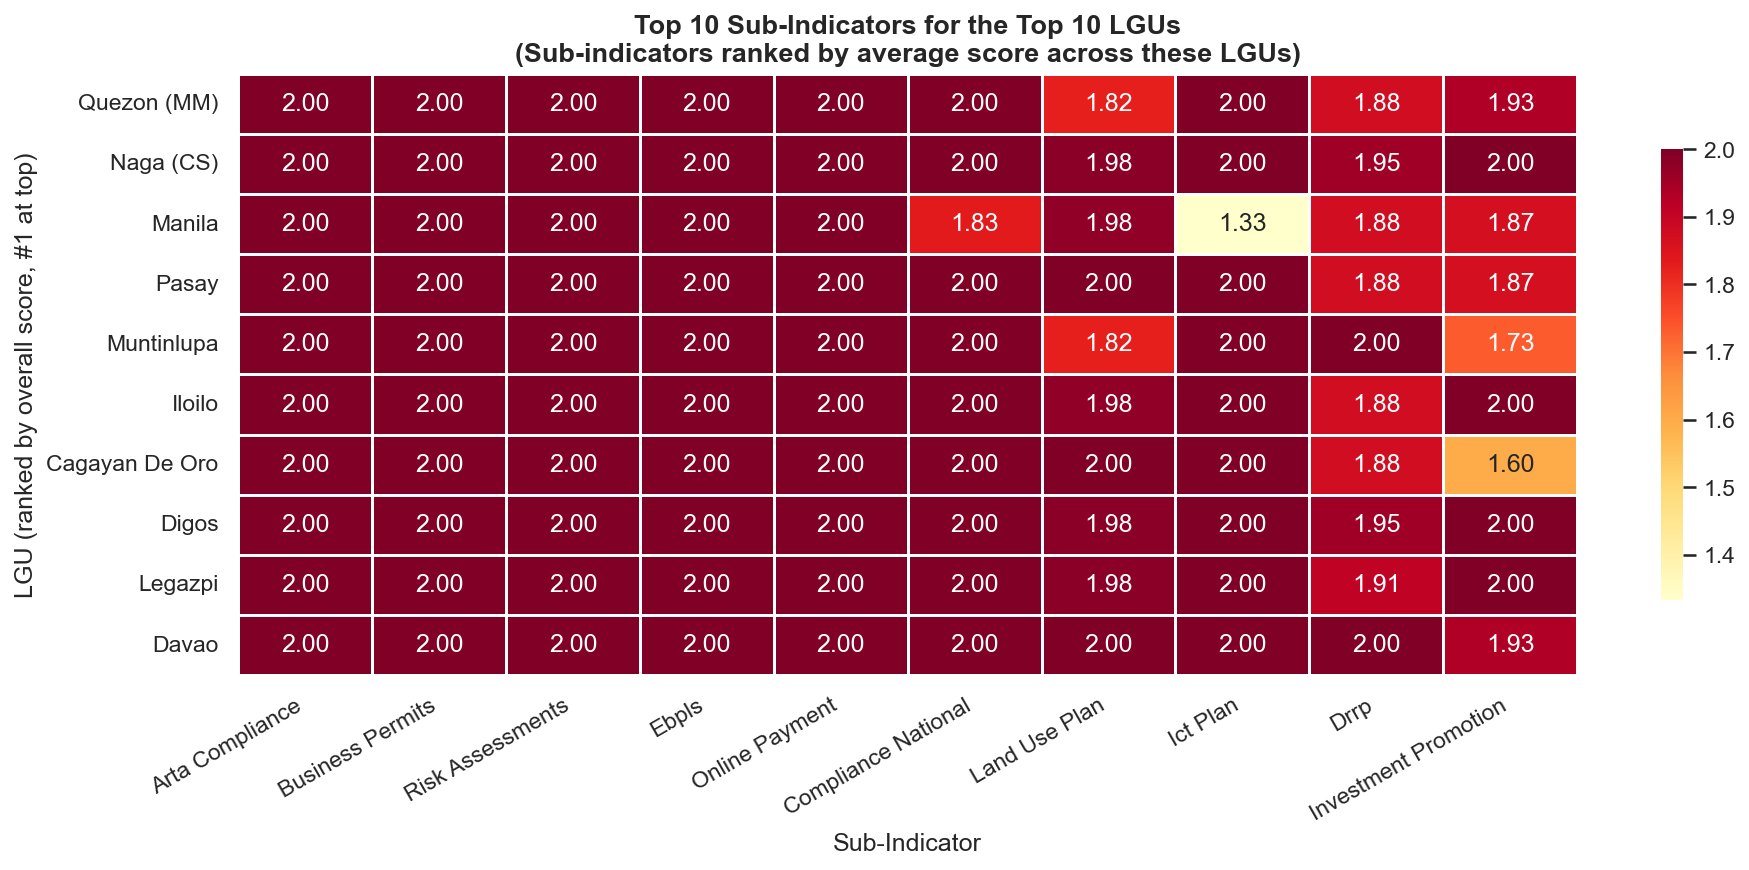
\includegraphics[width=\textwidth]{chart_02.png}
    \caption{Heatmap of the top 10 CMCI sub-indicator scores for the 10 highest-ranked LGUs. Values are uniformly high across all shown sub-indicators (darker = higher score), confirming that the best-performing LGUs do not rely on a single standout metric but score well across all dimensions.}
    \label{fig:top10_subind}
\end{figure*}

% ─────────────────────────────────────────────
\section{Discussion}
\label{sec:discussion}

\subsection{Three Tiers, Not Two}

A simple high/low split of competitiveness misses important structure. The Developing Mainstream cluster (64.8\% of LGUs) is genuinely different from both the Leaders and the Critically Underserved. It has Resiliency scores close to the Leaders tier (10.89 vs. 11.65) but Innovation scores only slightly above the Underserved tier (3.72 vs. 1.30). This suggests that Mainstream LGUs have built a foundation in disaster preparedness and basic services, but have not yet developed the technology and governance capacity needed to move up to the Leaders group.

\subsection{Innovation as the Ceiling, Resiliency as the Floor}

The pillar importance results in Fig.~\ref{fig:pillar_importance} point to a clear pattern: Innovation separates the top tier from the rest, while Resiliency deficits most strongly characterize the bottom tier. Infrastructure is never the top pillar for any tier. For the Leaders it ranks third (9.76), close behind Innovation (10.54) and Government Efficiency (9.94), which is consistent with top performers being strong across the board. For the two lower tiers, however, it ranks only fourth of five (1.32 for the Underserved and 0.29 for the Mainstream), well behind Resiliency and Government Efficiency for the Underserved tier and Innovation for the Mainstream tier. Infrastructure is part of what top performers have, but it is not what most clearly separates the lower tiers. Physical infrastructure investment alone is therefore unlikely to move an LGU between tiers; the bigger gains likely come from strengthening resiliency planning and governance and from building an innovation ecosystem.

\subsection{Compound Deprivation in the Underserved Tier}

One of the clearest findings is that Cluster 1 membership cannot be explained by failure in just one area. As the radar chart (Fig.~\ref{fig:radar}) and heatmap (Fig.~\ref{fig:cluster_heatmap}) both show, the 45 Critically Underserved LGUs score near the bottom across all five pillars at the same time. This means targeted, single-sector programs are unlikely to be enough. These communities need coordinated support across all five dimensions simultaneously.

\subsection{Model Limitations}

A few limitations are worth keeping in mind. First, the CMCI data is a single-year snapshot (2024), so we cannot track changes over time or draw causal conclusions. Second, K-Means assumes roughly spherical, similarly sized clusters, which may not fully capture the variety within the large Mainstream group. Third, the classifier is predicting labels that were generated by K-Means in the first place, so the high accuracy reflects internal consistency rather than validation against an independent ground truth.

% ─────────────────────────────────────────────
\section{Conclusion}
\label{sec:conclusion}

This paper applied a two-stage machine learning pipeline to the 2024 CMCI dataset covering 1,634 Philippine local government units. K-Means clustering with $k{=}3$, selected by both the elbow criterion and the silhouette score, identified three competitiveness tiers: 530 Competitive Leaders, 1,059 Developing Mainstream units, and 45 Critically Underserved municipalities. L1-penalized logistic regression trained on 50 raw sub-indicators reached 97.9\% test accuracy and 99.3\% full-dataset accuracy, showing that the tier structure is firmly encoded in the raw data. Innovation and Government Efficiency were the strongest predictors of top performance, while Resiliency deficits most clearly mark the underserved tier. A model-derived watchlist points to 15 municipalities in Sulu, Lanao del Sur, and Basilan as the highest-priority targets for intervention.

Based on these findings, we suggest three directions for policy: (1) invest in ICT infrastructure and STEM education in Cluster 2 municipalities to help them move toward the Leaders tier; (2) deploy coordinated, multi-pillar support programs in the 45 Critically Underserved LGUs rather than one-off sector projects; and (3) use the model's predicted probabilities as an ongoing screening tool for DTI and NEDA resource allocation. Extending this analysis to multiple years of CMCI data would make it possible to track tier mobility over time and better understand what actually causes municipalities to move up or down.

% ─────────────────────────────────────────────
\begin{thebibliography}{00}

\bibitem{cmci2024}
Department of Trade and Industry -- Philippines, ``Cities and Municipalities Competitiveness Index 2024,'' \textit{DTI CMCI Portal}, 2024. [Online]. Available: \url{https://cmci.dti.gov.ph/rankings-data.php}

\bibitem{lloyd1982}
S. P. Lloyd, ``Least squares quantization in PCM,'' \textit{IEEE Transactions on Information Theory}, vol. 28, no. 2, pp. 129--137, 1982.

\bibitem{macqueen1967}
J. MacQueen, ``Some methods for classification and analysis of multivariate observations,'' in \textit{Proc. 5th Berkeley Symposium on Mathematical Statistics and Probability}, 1967, vol. 1, pp. 281--297.

\bibitem{rousseeuw1987}
P. J. Rousseeuw, ``Silhouettes: A graphical aid to the interpretation and validation of cluster analysis,'' \textit{Journal of Computational and Applied Mathematics}, vol. 20, pp. 53--65, 1987.

\bibitem{tibshirani1996}
R. Tibshirani, ``Regression shrinkage and selection via the lasso,'' \textit{Journal of the Royal Statistical Society: Series B}, vol. 58, no. 1, pp. 267--288, 1996.

\bibitem{pedregosa2011}
F. Pedregosa et al., ``Scikit-learn: Machine learning in Python,'' \textit{Journal of Machine Learning Research}, vol. 12, pp. 2825--2830, 2011.

\bibitem{defazio2014}
A. Defazio, F. Bach, and S. Lacoste-Julien, ``SAGA: A fast incremental gradient method with support for non-strongly convex composite objectives,'' in \textit{Advances in Neural Information Processing Systems (NeurIPS)}, 2014, pp. 1646--1654.

\bibitem{pearson1901}
K. Pearson, ``On lines and planes of closest fit to systems of points in space,'' \textit{The London, Edinburgh, and Dublin Philosophical Magazine and Journal of Science}, vol. 2, no. 11, pp. 559--572, 1901.

\end{thebibliography}

\end{document}
